\documentclass[a4paper]{book}

%%% INICIO DEL PREÁMBULO %%%

\usepackage[utf8]{inputenc}
\usepackage[greek,spanish,es-tabla,es-nodecimaldot,es-noindentfirst]{babel}
\usepackage{babelbib}
\usepackage{nccmath}
\usepackage{amsthm}
\usepackage{lipsum}
\usepackage{tcolorbox}
\usepackage[thicklines]{cancel}
\usepackage{mathtools}
\usepackage{amssymb}
\usepackage{amsmath}
\usepackage{caption}
\usepackage{subcaption}
\usepackage{color}
\usepackage{verbatim}
\usepackage{enumerate}
\usepackage{geometry}
\geometry{a4paper,left=35mm,right=35mm,top=15mm,bottom=15mm}
\usepackage{isotope}
\usepackage{maybemath}
\usepackage{upgreek}
\usepackage{wasysym}
\usepackage[italic]{hepparticles}
\usepackage{subdepth}
\usepackage{siunitx}
\sisetup{
	mode 			= text,
	parse-units 	= false
}
\usepackage{physics}
\usepackage{braket}
\usepackage{tensor}
\usepackage{chemformula}
\usepackage{tikz}
\usepackage{url}
\usepackage{listings}
\usepackage{multirow}
\usepackage{multicol}
\usepackage[colorlinks=true]{hyperref}
\hypersetup{
	citecolor = blue,
	linkcolor = blue,
	urlcolor = blue,
	pdfauthor = {Javier Rodrigo López}
}
\usepackage{eso-pic}

% tikz
\usepackage{tikz} \usetikzlibrary{fit,babel,shapes,arrows,patterns,positioning,calc,decorations.pathmorphing,decorations.markings}
\tikzstyle{block} = [draw, fill=white, rectangle,
minimum height=3em, minimum width=6em]
\tikzstyle{sum} = [draw, fill=white, circle, node distance=1cm]
\tikzstyle{input} = [coordinate]
\tikzstyle{output} = [coordinate]
\tikzstyle{pinstyle} = [pin edge={to-,thin,black}]
\tikzset{
	block/.style = {draw, fill=white, rectangle, minimum height=3em, minimum width=3em},
	tmp/.style  = {coordinate},
	sum/.style= {draw, fill=white, circle, node distance=1cm},
	input/.style = {coordinate},
	output/.style= {coordinate},
	pinstyle/.style = {pin edge={to-,thin,black}}
}

\usepackage[oldvoltagedirection]{circuitikz}
\usepackage{pdflscape}

% Títulos
\usepackage{titlesec}
\titleformat{\section}{\normalfont\Large\bfseries}{\thesection}{1em}{}[{\titlerule[0.8pt]}]
% \renewcommand{\thesubsection}{\arabic{chapter}.\arabic{section}.\Alph{subsection}}
\titleformat{\subsubsection}{\normalfont\normalsize\bfseries}{\thesubsubsection}{1em}{}[{\titlerule[0.05pt]}]
\titlespacing{\section}{0pt}{2\parskip}{\parskip}
\titlespacing{\subsection}{0pt}{\parskip}{0pt}
\titlespacing{\subsubsection}{0pt}{\parskip}{0pt}

% Numeración de secciones
\setcounter{tocdepth}{2}
\setcounter{secnumdepth}{2}

% Figuras y descripciones
\renewcommand{\thefigure}{\arabic{figure}}
\renewcommand{\thesubfigure}{\Alph{subfigure}}
\captionsetup[figure]{labelfont={bf},name={Figura},labelsep=period}
\numberwithin{figure}{chapter}
\numberwithin{equation}{chapter}

% Enumerations
\newcounter{myenumi}
\renewcommand{\themyenumi}{\alph{myenumi})}
\newenvironment{myenumerate}{\setlength{\parindent}{0pt}\setcounter{myenumi}{0}\renewcommand{\item}{\par\refstepcounter{myenumi}\makebox[1.3em][l]{\themyenumi}}}{\par\bigskip\noindent\ignorespacesafterend}

% Own environments
\newenvironment{nota}{\underline{\textbf{NOTA:}} }{}
\newenvironment{caja}{\begin{tcolorbox}[colback = white, sharp corners, boxrule = 1 pt]}{\end{tcolorbox}}
\newtheorem*{conclusion}{Conclusión}
\newtheorem{teorema}{Teorema}
\newtheorem{definicion}{Definición}

% Para una bonita portada
\usepackage{wallpaper}
\usepackage{titling}
\usepackage{fancyhdr}
\pagestyle{fancy}
\setlength{\droptitle}{-10cm}
\renewcommand{\chaptermark}[1]{%
	\markboth{#1}{}}
\renewcommand{\sectionmark}[1]{%
	\markright{}}
\fancyhf{}
\fancyhead[LE,RO]{\bfseries\thepage} \fancyhead[LO]{\bfseries\rightmark} \fancyhead[RE]{\bfseries\leftmark} \renewcommand{\headrulewidth}{0pt} \renewcommand{\footrulewidth}{0pt} \addtolength{\headheight}{15pt}
\fancypagestyle{plain}{%
	\fancyhead{}
	\renewcommand{\headrulewidth}{0pt}
}

% Organización del texto
\newcommand{\formula}[1]{\vspace{13 pt}\noindent \textbf{\underline{#1}}}
\newcommand{\subtext}[1]{_{\text{#1}}}

% Unidades y utilidades varias
\renewcommand{\S}{\operatorname{S}}
\newcommand{\dB}{\operatorname{dB}}
\newcommand{\dBW}{\operatorname{dBW}}
\newcommand{\dBm}{\operatorname{dBm}}
\newcommand{\Hz}{\operatorname{Hz}}
\newcommand{\s}{\operatorname{s}}
\newcommand{\A}{\operatorname{A}}
\newcommand{\V}{\operatorname{V}}
\newcommand{\ohm}{\,\Omega}
\newcommand{\Pa}{\operatorname{Pa}}
\newcommand{\W}{\operatorname{W}}
\newcommand{\I}{\operatorname{I}}
\newcommand{\C}{\operatorname{C}}
\newcommand{\K}{\operatorname{K}}
\newcommand{\m}{\operatorname{m}}
\newcommand{\mm}{\operatorname{mm}}
\newcommand{\rad}{\operatorname{rad}}
\newcommand{\mol}{\operatorname{mol}}
\newcommand{\J}{\operatorname{J}}
\newcommand{\kg}{\operatorname{kg}}
\newcommand{\incremento}{\Delta}
\newcommand{\psus}{\, \ldots \,}
\newcommand{\mcm}{\operatorname{mcm}}
\newcommand{\MCD}{\operatorname{MCD}}
\renewcommand{\sin}{\sen}
\renewcommand{\arcsin}{\arcsen}
\renewcommand{\arctan}{\arctg}
\renewcommand{\min}{\operatorname{mín}}

\DeclarePairedDelimiter\evaluat{.}{\rvert}

% Vectores
\usepackage[c]{esvect}
\renewcommand{\vec}[1]{\vv{{#1}}}
\newcommand{\proy}[2]{\operatorname{proy}_{\vec{#2}}\vec{#1}}
\newcommand{\antiparallel}{\downharpoonleft \! \upharpoonright}
\newcommand{\parallelvec}{\upharpoonleft \! \upharpoonright}

% Espaciado
\usepackage{enumitem}
\setlist{before={\parskip=3pt}, after=\vspace{\baselineskip}}
\setlength{\parindent}{0pt}
\setlength{\parskip}{0.5em}

% Estadística
\DeclareMathOperator{\Var}{Var}
\DeclareMathOperator{\Cov}{Cov}
\renewcommand{\var}{\sigma ^2}
\DeclareMathOperator{\B}{B}
\DeclareMathOperator{\BN}{BN}
\DeclareMathOperator{\Geo}{Geo}
\DeclareMathOperator{\Poisson}{Poisson}
\DeclareMathOperator{\U}{U}
\DeclareMathOperator{\Exp}{Exp}
\DeclareMathOperator{\N}{N}
\DeclareMathOperator{\Mult}{Mult}
\newcommand{\TF}[1]{\mathrm{TF} \left\lbrace \left. #1 \right\rbrace \right.}
\newcommand{\probCond}[2]{P \left( #1 \: \middle\vert\:  #2 \right) }

% Electromagnetismo y Ondas
\newcommand{\errorGrave}{\textbf{FG!!!}}
\newcommand{\mas}{M.A.S.}
\newcommand{\mcu}{M.C.U.}
\newcommand{\ed}{E.D.}
\newcommand{\edmas}{E.D. del M.A.S.}
\usepackage{esint}

% Señales y Sistemas
\renewcommand{\H}{H}

% Circled number
\newcommand{\circledNumber}[1]{\raisebox{.9pt}{\textcircled{\raisebox{-.9pt}{#1}}}}

% Footnotes
% \renewcommand{\thefootnote}{\fnsymbol{footnote}}

% Ejemplo
\newcounter{elejemplo}
\newcommand{\ejemplo}[2]{
	\refstepcounter{elejemplo}
	\begin{center}
		\fbox{\begin{minipage}{0.85\linewidth}
			\textbf{Ejemplo \arabic{elejemplo}.} #1
			\begin{center}
				\underline{\textbf{Solución}}
			\end{center}
			#2
		\end{minipage}}
	\end{center}
}

% Repeticiones
\usepackage{forloop}
\newcommand{\repvec}[3]{
	\foreach \uwu in {1,...,#2}
		{\vec{#1}_{\uwu} ,}
	\, \ldots \, , \vec{#1}_{#3}
}
\newcommand{\rep}[3]{
	\foreach \uwu in {1,...,#2}
		{#1_{\uwu} ,}
	\, \ldots \, , #1_{#3}
}
\newcommand{\repinf}[3]{
	\foreach \uwu in {#2,...,#3}
		{#1_{\uwu} ,}
	\, \ldots
}

%%% FIN DEL PREÁMBULO %%% % Se incluye el preámbulo

% Título y portada
\title{\Huge Señales y Sistemas\\
\Large Apuntes de clase}
\author{Javier Rodrigo López \thanks{E-mail: \href{mailto:javiolonchelo@gmail.com}{\texttt{javiolonchelo@gmail.com}}} \and con ayuda de Hao Feng Chen Fu}
\date{\today}

%%% INICIO DEL DOCUMENTO %%%
\begin{document}

\setlength{\wpYoffset}{-1 cm}
\ThisCenterWallPaper{0.4}{./Imágenes/Van Gogh.jpg}
\maketitle

% Marca de agua
\AddToShipoutPictureFG{
	\begin{tikzpicture}[overlay,remember picture]
		\path (current page.south west) -- (current page.north east)
		node[midway,scale=8,color=lightgray,sloped,opacity=0.05] {Javier Rodrigo López};
	\end{tikzpicture}
}

% Logotipos UPM y ETSIST
\begin{figure}[t!]
	\centering
	\begin{subfigure}[b]{0.65\linewidth}
		
\includegraphics[width=\linewidth]{../../Archivos comunes/upm_logo.png}
	\end{subfigure}
	\begin{subfigure}[b]{0.25\linewidth}
		
\includegraphics[width=\linewidth]{../../Archivos comunes/etsist_logo.png}
	\end{subfigure}
\end{figure}

% Introducción
\newpage
\phantomsection
\addcontentsline{toc}{section}{Introducción}
\section*{Introducción}
\vspace{1em}
Esta pequeña recopilación de fórmulas, teoremas y demás apuntes de teoría ha sido elaborada durante el primer semestre del curso 2020-2021, en la escuela \href{https://www.etsist.upm.es/}{\textbf{ETSIST}} de la \href{http://www.upm.es/}{\textbf{UPM}} por Javier Rodrigo López, alumno de 2º de Ingeniería de Sonido e Imagen.

Una parte de este documento ha sido extraída de un libro subido a Wuolah por Javier Monasterio Solar (falta referencia). También han sido de gran ayuda los apuntes de Daniel Fernández Casado (quien, curiosamente, conoce mi pueblo) y el libro de Señales y Sistemas, de Oppenheim (añadir referencia), junto con sus clases grabadas del MIT OpenCourseWare.
\newpage

% Índice (TOC)
\setlength{\parskip}{0em}
\tableofcontents
\setlength{\parskip}{0.5em}

%%% INICIO DE LOS APUNTES %%%
\chapter{Introducción al análisis de señales en el dominio del tiempo}

\section{Señales: definición y clasificación}
Una \textbf{señal} es una función de una o más variables independientes que aporta información sobre algún fenómeno.

Las señales se pueden clasificar en:

\begin{enumerate}
	\item \textbf{Señales de tiempo continuo:} Son aquellas en las que las variables independientes toman valor para cualquier número real.
	\item \textbf{Señales de tiempo discreto:} Son aquellas en las que las variables independientes solo toman valores enteros.
\end{enumerate}


\section{Propiedades y transformaciones de la variable independiente}

\subsection{Propiedades de las señales}
Las señales, tanto las continuas como las discretas, son caracterizadas por unas ciertas propiedades:
\begin{enumerate}
\item \textbf{Simetría:} Una señal puede ser par, si $x(-t) = x(t)$; o impar, si $x(-t) = -x(t)$. Ten en cuenta que, para que haya simetría impar, se tiene que cumplir que $x(0) = 0$.
\item \textbf{Periodicidad:} Una señal es periódica si se repite cada cierto tiempo $T$, al cual llamamos \emph{periodo}. Matemáticamente: \[x(t) = x(t+T) \ \forall t \qquad T \in \mathbb{R}\]
\item \textbf{Causalidad:} \begin{itemize}
\item En tiempo continuo, una señal es causal si $x(t) = 0 \quad \forall t < 0$.
\item En tiempo discreto, una señal es causal si $x[n] = 0 \quad \forall n<0$.
\end{itemize}
\begin{nota}
La definición que hemos visto de causalidad solo nos sirve para las señales. Más adelante, veremos que la causalidad para sistemas se define de forma diferente.
\end{nota}
\end{enumerate}




\subsection{Desplazamiento}
Desplazar una señal significa moverla a lo largo del eje $x$ para situarla en un lugar determinado del mismo.

\begin{ejemplo}
	Teniendo una señal $x[n]$\footnote{Si es una señal discreta, va con corchetes y dentro de ellos se usa la letra $n$}, queremos construir $x_2[n]$, siendo: \[x_2[n] = x[n-3]\]
\end{ejemplo}

\begin{ejemplo}
	Además, queremos definir otra señal $x_3[n]$ tal que: \[x_3[n] = x[n+1]\]
\end{ejemplo}

Puedes ver la representación de estas señales en la \autoref{fig:señales_desplazadas}.


\begin{figure}[htb]
	\centering
	\caption{Señales desplazadas}
	\begin{subfigure}[b]{0.45\textwidth}
		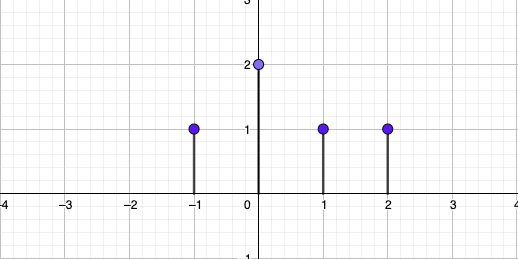
\includegraphics[width=\textwidth]{./Imágenes/aaa.png}
		\subcaption{Señal original $x[n]$.}
	\end{subfigure}
	\hfill
	\begin{subfigure}[b]{0.45\textwidth}
		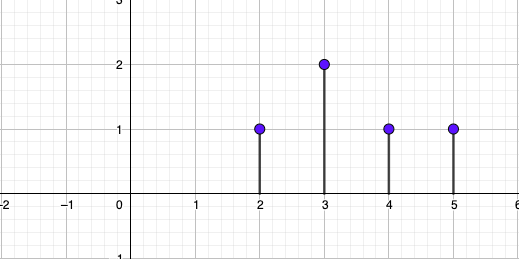
\includegraphics[width=\textwidth]{./Imágenes/aac.png}
		\subcaption{Señal desplazada a la izquierda $x_2[n]$.}
	\end{subfigure}

	\begin{subfigure}[b]{0.45\textwidth}
		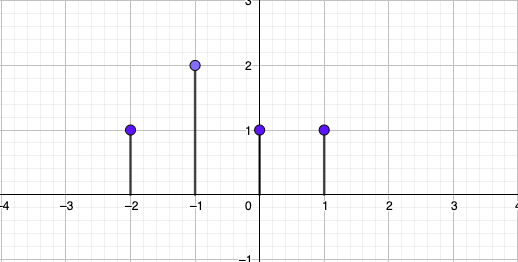
\includegraphics[width=\textwidth]{./Imágenes/aab.png}
		\subcaption{Señal desplazada a la derecha $x_3[n]$.}
	\end{subfigure}
	\label{fig:señales_desplazadas}
\end{figure}


\subsubsection{Conclusión}
\[\left\{ \begin{array}{l c l}
		\! \! \textrm{Si se suma una cantidad}  & \longrightarrow & \textrm{Desplazamiento a la izquierda} \\
		\! \! \textrm{Si se resta una cantidad} & \longrightarrow & \textrm{Desplazamiento a la derecha}
	\end{array} \right.
\]

\begin{nota}
	Las señales de tiempo continuo cumplen lo mismo, aunque sus desplazamientos no tienen por qué ser cantidades enteras.
\end{nota}

\subsection{Reflexión}

Reflejar una señal darle la vuelta (como si estuviera en espejo) con respecto al eje vertical.

\begin{ejemplo}
	Teniendo $x[n]$, se desea construir $x_2[n]$ tal que: \[x_2[n] = x[-n] \]
\end{ejemplo}

\begin{ejemplo}
	De la misma forma, se puede definir la reflexión para una señal continua $x(t)$, obteniéndose así la función $x_2(t)$ tal que: \[x_2(t) = x(-t)\]
\end{ejemplo}

Puedes ver la representación de estas señales en la \autoref{fig:señales_reflejadas}.


\begin{figure}[htb]
	\centering
	\caption{Señales reflejadas}

	\hfill
	\begin{subfigure}[t]{0.4\textwidth}
		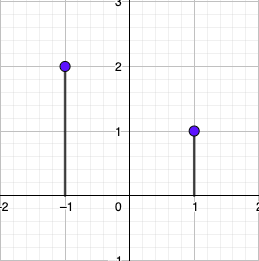
\includegraphics[width=\textwidth]{./Imágenes/aad.png}
		\subcaption{Señal discreta original $x[n]$.}
	\end{subfigure}
	\hfill
	\begin{subfigure}[t]{0.4\textwidth}
		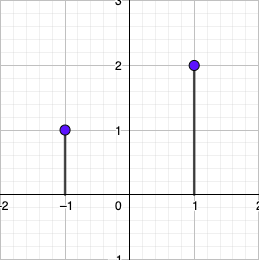
\includegraphics[width=\textwidth]{./Imágenes/aae.png}
		\subcaption{Señal discreta reflejada $x_2[n]$.}
	\end{subfigure}
	\hfill

	\vspace{5 pt}

	\hfill
	\begin{subfigure}[b]{0.4\textwidth}
		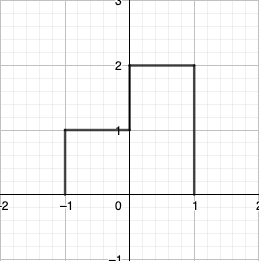
\includegraphics[width=\textwidth]{./Imágenes/aaf.png}
		\subcaption{Señal continua original $x(t)$.}
	\end{subfigure}
	\hfill
	\begin{subfigure}[b]{0.4\textwidth}
		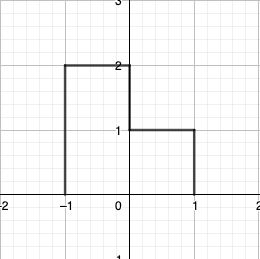
\includegraphics[width=\textwidth]{./Imágenes/aag.png}
		\subcaption{Señal continua reflejada $x_2(t)$.}
	\end{subfigure}
	\hfill

	\label{fig:señales_reflejadas}
\end{figure}

\subsection{Cambio de escala}

El cambio de escala de una señal se consigue multiplicando la variable independiente de la misma por una constante $\lambda \in \mathbb{R}$ , tal que:

\[\left\{ \begin{array}{l c l}
\textrm{Si } \lambda > 1 & \longrightarrow & \textrm{Operación de compresión} \\
\textrm{Si } \lambda < 1 & \longrightarrow & \textrm{Operación de expansión}
\end{array} \right.
\]

\begin{ejemplo}
	Dada una señal $f(t)$, se construye una señal $g(t)$ tal que: \[g(t) = f(2t) \quad \textrm{(Compresión)} \]
\end{ejemplo}

\begin{ejemplo}
	Dada una señal $f(t)$, se construye una señal $h(t)$ tal que: \[g(t) = f(0.5t) \quad \textrm{(Expansión)}\]
\end{ejemplo}

Puedes ver la representación de estas señales en la \autoref{fig:cambio_de_escala}.


\begin{figure}[!ht]
	\centering
	\caption{Señales continuas con cambios de escala}
	\begin{subfigure}[b]{0.45\textwidth}
		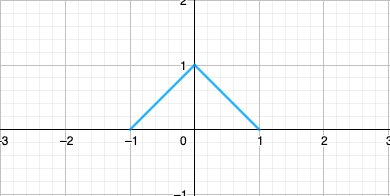
\includegraphics[width=\textwidth]{./Imágenes/aah.png}
		\subcaption{Señal original $f(t)$.}
	\end{subfigure}
	\hfill
	\begin{subfigure}[b]{0.45\textwidth}
		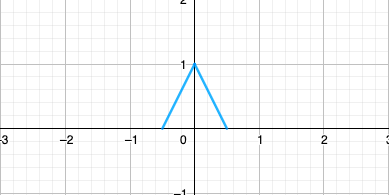
\includegraphics[width=\textwidth]{./Imágenes/aai.png}
		\subcaption{Señal comprimida $g(t) = f(2t)$.}
	\end{subfigure}

	\begin{subfigure}[b]{0.45\textwidth}
		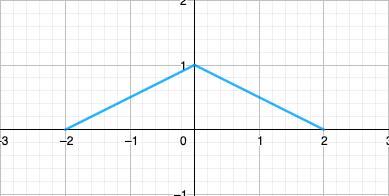
\includegraphics[width=\textwidth]{./Imágenes/aaj.png}
		\subcaption{Señal ampliada $h(t) = f(0.5t)$.}
	\end{subfigure}
	\label{fig:cambio_de_escala}
\end{figure}


La operación del cambio de escala no es reversible en señales discretas. Por eso mismo, diferenciamos dos operaciones diferentes:
\begin{enumerate}
\item \textbf{Operación de diezmado:} Es equivalente a comprimir la señal. Necesariamente se pierde información en este proceso, ya que habrá ciertas muestras de la señal ($t=1$, por ejemplo) que acabarán en lugares donde, por ser una señal discreta, no puede haber información ($t=0.5$, ya que $0.5 \not \in \mathbb{Z}$).
\item \textbf{Operación de interpolación:} Equivale a expandir la señal. Aquellas partes de la señal donde se perdió información durante el diezmado (o donde simplemente no había) ahora reaparecen como muestras de valor 0. Matemáticamente, se define como: \[y[n] \left\{ \begin{matrix*}[l]
x\left[ \frac{n}{2} \right] & \text{si } n \text{ es par} \\
0 & \text{si } n \text{ es impar}
\end{matrix*} \right. \]
\end{enumerate}

Puedes ver los cambios de escala de las señales discretas en la \autoref{fig:cambio_de_escala_discreto}.


\begin{figure}[!ht]
	\centering
	\caption{Señales discretas con cambios de escala}
	\begin{subfigure}[b]{0.4\textwidth}
		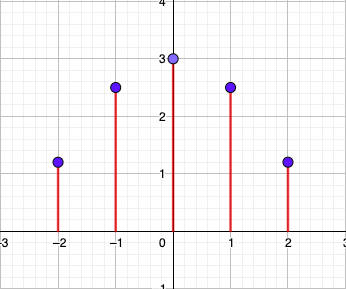
\includegraphics[width=\textwidth]{./Imágenes/aak.png}
		\subcaption{Señal original.}
	\end{subfigure}
	\hfill
	\begin{subfigure}[b]{0.4\textwidth}
		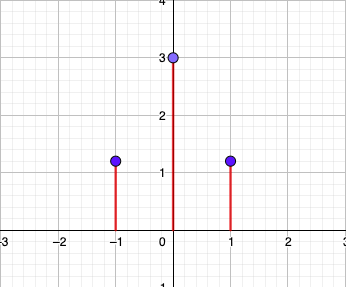
\includegraphics[width=\textwidth]{./Imágenes/aal.png}
		\subcaption{Señal diezmada.}
	\end{subfigure}

	\begin{subfigure}[b]{0.7\textwidth}
		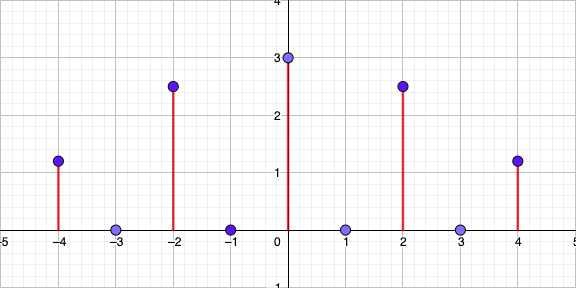
\includegraphics[width=\textwidth]{./Imágenes/aam.png}
		\subcaption{Señal interpolada.}
	\end{subfigure}
	\label{fig:cambio_de_escala_discreto}
\end{figure}


\newpage
\section{Estudio de las señales básicas}
\subsection{Energía}

La \textbf{energía} de una señal $x(t)$ en el intervalo de tiempo $\left( t_1, t_2 \right)$ se define como: \[E_x=\int_{-t_1}^{t_2}{\abs{x(t)}^2\dd t}\]

Si se trata de una señal discreta $x[n]$ en el intervalo de tiempo $\left[ n_1, n_2 \right]$, entonces se define como: \[E_x=\sum^{n_2}_{n=n_1}{\abs{x[n]}^2}\]

\subsection{Potencia}
A veces, puede que tratemos con señales que resulten tener energía infinita. En esos casos es probable que sea más útil tener en cuenta la \textbf{potencia} de la señal.
\vspace{10 pt}

{\centering

\underline{En tiempo \textbf{continuo}}
\begin{multicols}{2}
$\boxed{\text{Señal periódica}}$
\[P_x=\frac{1}{T}\int_{-\frac{T}{2}}^{\frac{T}{2}}{\abs{x(t)}^2\dd t}\]
$\boxed{\text{Señal no periódica}}$
\[P_x=\lim_{T \to \infty}{\left( \frac{1}{T}\int^{\frac{T}{2}}_{-\frac{T}{2}}{\abs{x(t)}^2\dd t} \right)}\]
\end{multicols}

\underline{En tiempo \textbf{discreto}}
\begin{multicols}{2}
$\boxed{\text{Señal periódica}}$
\[P_x=\frac{1}{N}\sum_{n=N}{\abs{x[t]}^2}\]
$\boxed{\text{Señal no periódica}}$
\[P_x=\lim_{N \to \infty}{\left( \frac{1}{2N}\sum^{N-1}_{n=-N}{\abs{x[n]}^2} \right) }\]
\end{multicols}}


\subsection{Señales destacadas}
\subsubsection{Señal escalón}
La señal escalón se define de la siguiente manera:
\begin{multicols}{2}
\centering
En tiempo \textbf{continuo}
\[u(t) = \left\{ \begin{matrix*}[l]
1 & \text{si }t\geq 0 \\[5pt]
0 & \text{si }t <0
\end{matrix*} \right.\]

En tiempo \textbf{discreto}
\[u[n] = \left\{ \begin{matrix*}[l]
1 & \text{si }n\geq 0 \\[5pt]
0 & \text{si }n <0
\end{matrix*} \right.\]
\end{multicols}

\subsubsection{Señal impulso}
La señal impulso se define de la siguiente manera:
\begin{multicols}{2}
\centering
En tiempo \textbf{continuo} (delta de Dirac)
\[\delta (t) = \left\{ \begin{matrix*}[l]
\infty & \text{si }t = 0 \\[5pt]
0 & \text{si }t \not = 0
\end{matrix*} \right.\]

En tiempo \textbf{discreto} (delta de Kronecker)
\[\delta [n] = \left\{ \begin{matrix*}[l]
1 & \text{si }n = 0 \\[5pt]
0 & \text{si }n \not = 0
\end{matrix*} \right.\]
\end{multicols}

En realidad, en tiempo continuo se puede definir de una manera bastante más intuitiva. Si consideramos la señal escalón $u_\Delta (t)$ como la señal representada en la \autoref{subfig:escalon}, entonces podemos definir la señal impulso como: \[\delta _\Delta (t) = \dv{t} u_\Delta (t)\]


\begin{figure}[!ht]
	\caption{}
	\label{fig:escalon_e_impulso}
	\centering
	\begin{subfigure}[b]{0.45\linewidth}
		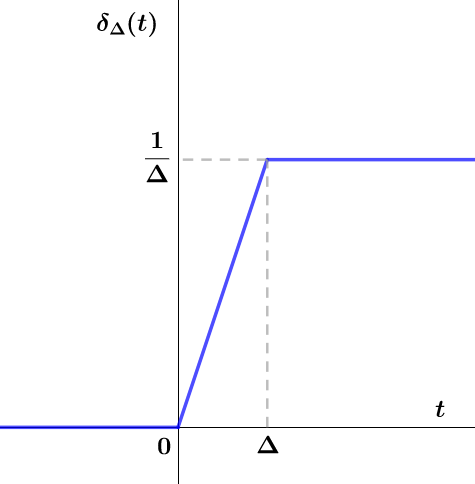
\includegraphics[width=\linewidth]{./Imágenes/aas.png}
		\subcaption{Señal escalón.}
		\label{subfig:escalon}
	\end{subfigure}
	\hfill
	\begin{subfigure}[b]{0.45\linewidth}
		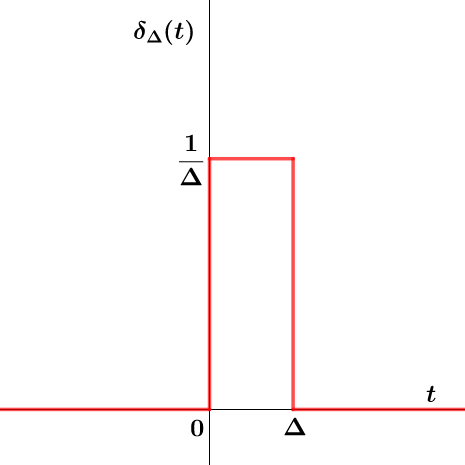
\includegraphics[width=\linewidth]{./Imágenes/aat.png}
		\subcaption{Señal impulso.}
		\label{subfig:impulso}
	\end{subfigure}
\end{figure}

Puedes ver la señal impulso en la \autoref{subfig:impulso}. Analíticamente, quedaría de esta forma: \[\delta _{\Delta}(t) = \left\{ \begin{matrix}
\dfrac{1}{\Delta} &  & \text{si }0<t<\Delta \\[12pt]
0                 &  & \text{en otro caso}
\end{matrix} \right.\]

Si nos fijamos, podemos notar que el área que encierra $\delta _\Delta (t)$ se puede calcular como el área de un rectángulo: base por altura. Es decir, \[A= \Delta\cdot \frac{1}{\Delta} = 1 \qquad \forall \Delta \in \mathbb{R} -\left\{ 0 \right\} \]

Teniendo eso en cuenta, definimos la delta de Dirac como: \[\delta (t) = \lim_{\Delta \to 0}{\delta _{\Delta} (t)}\]

De forma que podemos afirmar que:
\[\int_{-\infty}^\infty{\delta (t)\dd t} = 1\]


\begin{nota}
	\label{relacion_delta_escalon}
	La relación entre estas dos señales es muy importante. Si pensamos un poco, es fácil llegar a las siguientes conclusiones (aunque algunas ya las hemos visto, de otra forma):
	\begin{multicols}{2}
		\centering
		En tiempo \textbf{continuo}
		\[\delta (t) = \dv{u(t)}{t} \]
		\[u(t) = \int_{-\infty}^{t}{\delta (\tau ) \dd \tau }\]

		En tiempo \textbf{discreto}
		\[\delta [n] = u[n] - u[n-1]\]
		\[u[n] = \sum^{n}_{m=-\infty}{\delta [m]}\]
	\end{multicols}
\end{nota}

\begin{center}
	\underline{\textbf{Propiedades de la función delta de Dirac}}
	\begin{align*}
		x(t)\delta (t-t_0) = x(t_0)\delta(t-t_0) \\
		\text{Otras que aún no he puesto, sorry owo}
	\end{align*}
\end{center}

\subsubsection{Señal exponencial compleja}
Esta es una señal compleja que puede ser entendida como una modulación de una exponencial imaginaria por una exponencial real. \[x(t) = Ae^{rt}e^{j\left( \omega t + \beta \right)}\]

Esta señal tiene oscilaciones amortiguadas si $r<0$, o bien oscilaciones crecientes si $r>0$. (Insertar imágenes)

\subsubsection{Señal exponencial discreta}
Sean $A,\alpha ,\beta \in \mathbb{C}$ de modo que $\alpha = e^\beta $, entonces definimos la señal exponencial discreta como: \[x[n] = A\alpha ^n\]

Se puede distinguir entre:
\begin{enumerate}
\item Secuencia exponencial real: $A, \alpha \in \mathbb{R}$
\item Secuencia sinusoidal: $\abs{\alpha} = 1 \longrightarrow \alpha = e^{j\Omega}$
\item Secuencia con oscilaciones de amplitud variable: $\abs{\alpha} \not =1,\ \Im(\alpha) \not =0$
\end{enumerate}

\subsubsection{Señal sinusoidal discreta}
\[x[n] = e^{j\Omega n}\]

Esta señal es periódica si y solo si se cumple que: \[\Omega _0 = \frac{2\pi m}{N}\]

\chapter{Análisis de sistemas en el dominio del tiempo}

\section{Definición de sistema y de sus propiedades}
Se entiende por sistema cualquier transformación de una señal (que llamamos \textbf{señal de entrada}) en otra señal (que llamamos \textbf{señal de salida}).

Podemos expresar la relación entre la entrada y la salida como una expresión matemática que exprese la salida como función de la entrada del sistema:
\[y(t) = f\left\lbrace x(t) \right\rbrace \qquad \qquad y[n] = f\left\lbrace x[n] \right\rbrace\]

\subsection{Interconexión de sistemas}
\begin{itemize}
	\item En serie o cascada.
	\item En paralelo.
	\item De realimentación.
\end{itemize}

\subsection{Propiedades de los sistemas}
\begin{itemize}
\item \textbf{Linealidad}

Se refiere a la \textbf{proporcionalidad} del sistema.

Teniéndose dos entradas $x_1(t)$ y $x_2(t)$, y sus correspondientes salidas $y_1(t)$ e $y_2(t)$, si consideramos una tercera señal $x_3(t)$ que sea una combinación lineal de las otras dos entradas, la salida $y_3(t)$ será también una combinación lineal de las salidas $y_1(t)$ e $y_2(t)$.

Es decir: \[\text{Si } x_3(t) = ax_1(t) + bx_2(t) , \text{ entonces: }\ y_3(t) = y_3(t) = ay_1(t) + by_2(t) \qquad a,b\in \mathbb{R}\]

\item \textbf{Invarianza en el tiempo}

Un sistema es invariante en el tiempo si, como su propio título indica, el instante en el que la señal es procesada no afecta a la salida.

Siendo $y(t)$ la salida correspondiente a la entrada $x(t)$, la invarianza en el tiempo también se puede expresar como: \[x(t)= x_o(t-t_0) \ \Longrightarrow \ y(t)=y_0(t-t_0) \qquad \forall x_0(t), t_0\]


\item \textbf{Causalidad}

Un sistema es \textbf{causal} (también llamado \textsl{no anticipativo}) si la salida depende únicamente del estado actual del circuito o de estados pasados.

\underline{\textbf{Ejemplos:}}
\begin{itemize}
\item Un sistema causal es $y[n] = x[n-3]$.
\item Un sistema no causal es $y[n] = x[-n]$
\end{itemize}

\item \textbf{Memoria}

En un sistema \textbf{sin memoria}, la salida únicamente depende del estado actual del sistema. Por el contrario, en un sistema \textbf{con memoria}, la salida puede depender de situaciones pasadas o futuras del sistema.

Es decir, un sistema con relación entrada-salida $y(t) = 3x(t)$ no tiene memoria, pero uno con relación $y(t) = x(t-3)$ sí que tiene memoria.

\item \textbf{Estabilidad}

Se dice que un sistema es estable si para cualquier entrada acotada, la salida también es acotada.
\begin{itemize}
\item Si tomamos como ejemplo el sistema con relación entrada-salida $y(t) = tx(t)$, podemos asignar un valor arbitrario para $x(t)$ y observar si la salida está limitada. \[x(t) = 1 \qquad \Longrightarrow \qquad y(t) = t\]

Vemos que la salida puede crecer de forma ilimitada, por lo que este sistema no es estable.
\item Si, por otra parte, tomamos el sistema con relación $y(t) = e^{x(t)}$, podemos verificar su estabilidad asignando un valor límite de $x(t)$, de modo que: \[\abs{x(t)} < k \qquad \Longrightarrow \qquad \abs{y(t)} < e^k\]

Y vemos que la salida, al igual que la entrada, también está acotada. Así podemos afirmar que el sistema es estable.
\end{itemize}


\item \textbf{Invertibilidad}

En un sistema \textbf{invertible}, se puede determinar unívocamente qué entrada hubo según la salida que obtenemos.

Un sistema que cumple $y(t) = x^2(t)$ no es invertible, ya que no podemos saber qué signo hubo a la entrada solamente mirando en la salida. Por su parte, $y(t) = 2x(t)$ sí que es invertible, de modo que el sistema inverso resulta $w(t) = \frac{1}{2}y(t)$. \[w \left[ x(t) \right] = \frac{1}{2}\,  y\left[ x(t) \right] = \frac{1}{2}\, 2\, x(t) = x(t) \quad \longrightarrow \quad \boxed{ w \left[ x(t) \right] = x(t)}\]

\end{itemize}

\underline{\textbf{Algunas conclusiones importantes:}}
\begin{itemize}
	\item Todos los sistemas sin memoria son causales.
	\item Un sistema sin memoria no almacena energía/información/datos.
	\item Un sistema no causal siempre tiene memoria
\end{itemize}





\section{Sistemas LTI}
Por ahora, veremos solo sistemas \textbf{LTI} (lineales e invariantes en el tiempo).


\section{Representación de señales en términos de impulsos}
Si introducimos la señal impulso como entrada en un sistema, obtenemos una salida $h[n]$ que denominamos \textbf{respuesta al impulso}. Con ella podemos caracterizar completamente una señal LTI.

Entonces, tenemos que la relación entrada-salida del sistema viene dada por la \textbf{integral (o suma) de convolución}, y es:
\begin{align*}
	\text{Tiempo discreto: } & \qquad \boxed{y[n]=x[n]*h[n]=\sum^{\infty}_{m=-\infty}{x[k]h[n-k]}}    \\
	\text{Tiempo continuo: } & \qquad \boxed{y(t)=x(t)*h(t)=\int^{\infty}_{-\infty}{x(k)h(t-k)}\dd k}
\end{align*}

\subsection{Cálculo de la suma de convolución}
Vamos a realizar un ejercicio para ver cómo debemos hacer una suma de convolución en la práctica.
\vspace{\parskip}

\setlength{\leftskip}{0.5cm}
\setlength{\rightskip}{0.5cm}

\underline{\textbf{Problema 2 - Examen del 21 de enero de 2011}}

Dado un sistema LTI cuya respuesta al impulso es $h[n] = \delta [n+1] + \delta [n] + \delta [n-1]$:

Obtener razonadamente y representar gráficamente la salida para la entrada de la \autoref{fig:Problema_2_a} operando en el dominio del tiempo.

\begin{figure}[!ht]
	\caption{}
	\label{fig:Problema_2_a}
	\centering
	\begin{subfigure}[b]{0.75\linewidth}
		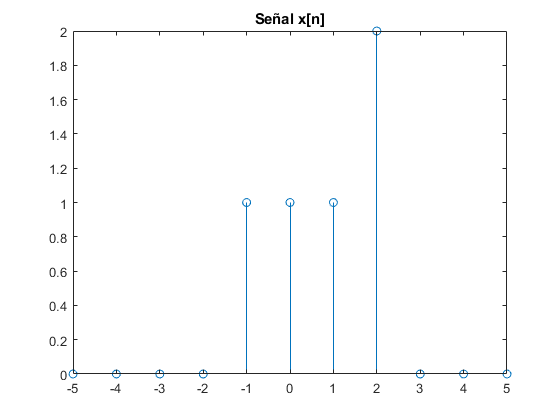
\includegraphics[width=\linewidth]{./Imágenes/aao.png}
	\end{subfigure}


\end{figure}

\vspace{\parskip}
\textbf{Solución:}

Primero obtenemos la señal $x[n]$, que se puede sacar a simple vista. \[x[n] = \delta [n+1] + \delta [n] + \delta [n-1] + 2 \delta [n-2]\]

\begin{figure}[!ht]
	\caption{}
	\label{fig:Problema_2_b}
	\centering
	\begin{subfigure}[b]{0.7\linewidth}
		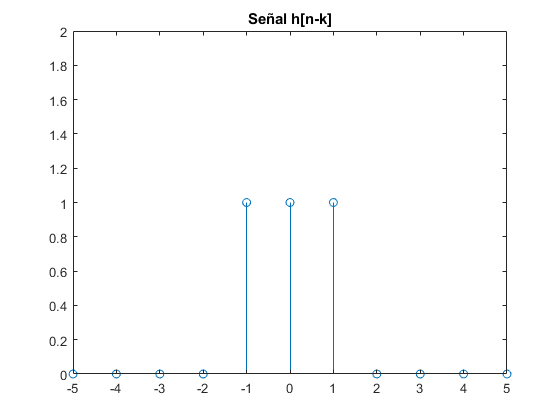
\includegraphics[width=\linewidth]{./Imágenes/aap.png}
	\end{subfigure}
\end{figure}

El siguiente paso será realizar la suma de convolución como tal. Aunque existen varias formas de hacerlo, yo explicaré la que a mí me parece más sencilla.

Ahora podríamos pensar que, por la definición de la convolución discreta, debemos dar la vuelta a una señal... ¡Pero no! Con este método no hace falta.

Tienes que seguir estos pasos:

\begin{enumerate}
\item Calcular el \textbf{instante inicial} de $y[n]$ (el primer valor de $n$ para el cual la salida será no nula). Este será la suma de los instantes iniciales de las señales a convolucionar.

En este caso, $h[n]$ empieza en $n=-1$. Si miramos $x[n]$, vemos que también empieza en $n=-1$.

Por lo tanto, el instante inicial de $y[n]$ será: \[n_0\footnotemark = (-1)+(-1) = -2\]
\footnotetext{Llamar $n_0$ al instante inicial de la señal no es ninguna notación concreta. Puede que no sea la forma más adecuada de nombrarlo, pero es la que se me ha ocurrido.}

\item \textbf{Realizar la pseudo-multiplicación.} La llamo así porque se parece bastante a una multiplicación de toda la vida, pero con la diferencia de que . Primero, vamos a escribir las señales de una forma más cómoda: \[\left\lbrace \begin{matrix*}[l]
x[k] &=& [\begin{matrix} 1 & \underline{1}& 1 &2 \end{matrix} ]\\[5pt]
h[n-k] &=& [\begin{matrix} 1 & \underline{1}& 1 \end{matrix} ]
\end{matrix*} \right. \qquad (\text{la línea indica el valor para }n=0)\]

Ahora, alinearemos el último elemento de $h[k]$ con el primero de $x[k]$. Debería quedar así:
\[ \begin{array}{ccccccc}
&   &               & 1 & \underline{1} & 1 & 2 \\
\circledast & 1 & \underline{1} & 1 &               &   &   \\
\hline
\end{array}
\begin{array}{|l}
\sim x[k] \\
\sim h[k]
\end{array}\]

Después de esto, realizaremos la pseudo-multiplicación. Escogemos el primer número de $h[k]$ y lo multiplicamos por cada elemento de $x[k]$. Los colocamos como se muestra a continuación:

\[ \begin{array}{ccccccc}
&                   &               & 1 & \underline{1} & 1 & 2 \\
\circledast & \circledNumber{1} & \underline{1} & 1 &               &   &   \\
\hline
& 1                 & 1             & 1 & 2             &   &   \\
&                   &               &   &               &   &   \\
&                   &               &   &               &   &
\end{array}
\begin{array}{|l}
\sim x[k]   \\
\sim h[k]   \\
\phantom{a} \\
\phantom{a} \\
\phantom{a}
\end{array}\]

Repetimos con el segundo número:

\[ \begin{array}{ccccccc}
&   &                               & 1 & \underline{1} & 1 & 2 \\
\circledast & 1 & \circledNumber{\underline{1}} & 1 &               &   &   \\
\hline
& 1 & 1                             & 1 & 2             &   &   \\
&   & 1                             & 1 & 1             & 2 &   \\
&   &                               &   &               &   &
\end{array}
\begin{array}{|l}
\sim x[k]   \\
\sim h[k]   \\
\phantom{a} \\
\phantom{a} \\
\phantom{a}
\end{array}\]

Y repetimos esto hasta haber hecho la multiplicación con todos los números de $h[n-k]$. Solo nos queda una última vez.

\[ \begin{array}{ccccccc}
&   &               & 1                 & \underline{1} & 1 & 2 \\
\circledast & 1 & \underline{1} & \circledNumber{1} &               &   &   \\
\hline
& 1 & 1             & 1                 & 2             &   &   \\
&   & 1             & 1                 & 1             & 2 &   \\
&   &               & 1                 & 1             & 1 & 2 \\
\end{array}
\begin{array}{|l}
\sim x[k]   \\
\sim h[k]   \\
\phantom{a} \\
\phantom{a} \\
\phantom{a}
\end{array}\]

Para concluir esta operación, simplemente sumamos los términos en cada columna, y obtenemos la secuencia $y[n]$.

\[ \begin{array}{ccccccc}
&            &               & 1          & \underline{1} & 1          & 2          \\
\circledast & 1          & \underline{1} & 1          &               &            &            \\
\hline
& 1          & 1             & 1          & 2             &            &            \\
&            & 1             & 1          & 1             & 2          &            \\
+           &            &               & 1          & 1             & 1          & 2          \\
\hline
& \mathbf{1} & \mathbf{2}    & \mathbf{3} & \mathbf{4}    & \mathbf{3} & \mathbf{2} \\
\end{array}
\begin{array}{|l}
\sim x[k]   \\
\sim h[k]   \\
\phantom{a} \\
\phantom{a} \\
\phantom{a} \\
\mathbf{\sim y[n]}
\end{array}\]
\end{enumerate}

Para concluir, recordamos que el instante inicial de $y[n]$ era $n_0=-2$. Esto nos permite escribir la señal de salida como: \[y[n] = \mathbf{1}\delta (n+2) + \mathbf{2}\delta (n+1) + \mathbf{3}\delta (n) + \mathbf{4}\delta (n-1) + \mathbf{3}\delta (n-2) + \mathbf{2}\delta (n-3)\]

\begin{figure}[!ht]
\caption{}
\label{fig:Problema_2_c}
\centering
\begin{subfigure}[b]{0.7\linewidth}
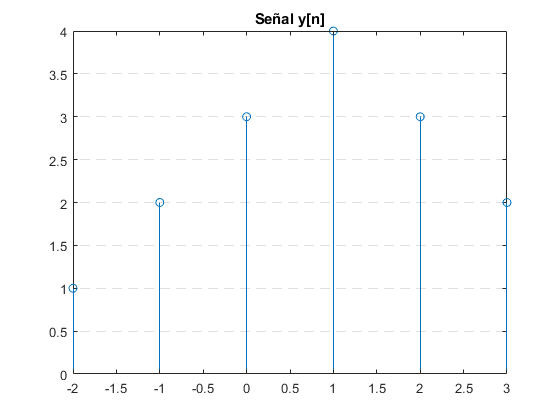
\includegraphics[width=\linewidth]{./Imágenes/aaq.png}
\end{subfigure}
\end{figure}

\setlength{\leftskip}{0pt}
\setlength{\rightskip}{0pt}

\subsection{Cálculo de la integral de convolución}
Al igual que antes, vamos a explicarlo mediante un ejercicio para saber desenvolvernos con facilidad en los problemas a los que nos enfrentemos. Y, ya que estamos, lo resolvemos entero, para ir cogiendo soltura.
\vspace{\parskip}


\setlength{\leftskip}{0.5cm}
\setlength{\rightskip}{0.5cm}

\underline{\textbf{Problema  - Examen final del 2 de julio de 2015}}\\[\parskip]
\begin{myenumerate}
La respuesta al impulso de un sistema LTI es el resultado de la siguiente convolución:
\[h(t) = u(t) \circledast \left( \delta (t+2) - \delta (t-1) \right)\]
\item  Obtener el resultado de la convolución y representar gráficamente la señal $h(t)$.
\item Representar gráficamente la siguiente señal:
\[x_1(t) = \abs{t-1}\cdot \left( u(t+1) - u(t-1) \right)\]

\item Representar gráficamente la siguiente señal: \[x_2(t) = x_1(-t-2)-x_1\left( \frac{1}{2}t -1 \right)\]

\item Calcular y representar gráficamente la salida $y(t)$ que proporciona el sistema de respuesta al impulso $h(t)$ cuando la señal de entrada es $x_1(t)$.
\end{myenumerate}

\vspace{\parskip}
\textbf{Solución:}
\begin{myenumerate}
\item El resultado de este apartado es inmediato si recordamos la relación que tienen la señal impulso y la señal escalón (\ref{relacion_delta_escalon}).
\[h(t) = u(t) \circledast \left[ \delta (t+2) - \delta (t-1) \right] = \boxed{u(t+2) - u(t-1)}\]

Solo nos queda representar $h(t)$:
\begin{figure}[!ht]
\caption{}
\label{fig:Problema_1_a}
\centering
\begin{subfigure}[b]{0.7\linewidth}
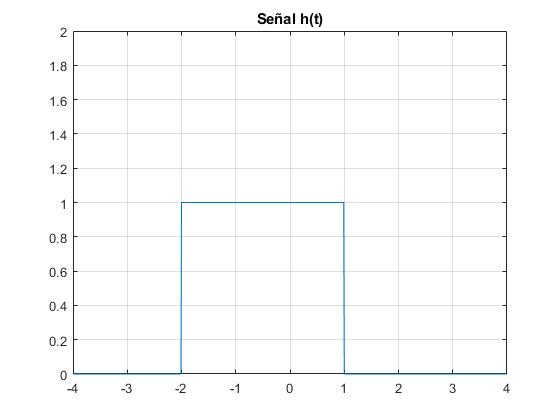
\includegraphics[width=\linewidth]{./Imágenes/aar.png}
\end{subfigure}
\end{figure}
\item Recordemos la señal con la que trabajaremos: \[x_1(t) = \abs{t-1}\cdot \left( u(t+1) - u(t-1) \right)\]

Si nos fijamos en las señales escalónsta señal es no nula para $-1\leq t<1$. Viendo que tiene un valor absoluto, vamos a redefinirla como una función a trozos. Si calculamos cuándo es negativo lo que se encuentra dentro del valor absoluto, veremos que la función a trozos quedará así:
\[x_1(t) = \left\{ \begin{matrix*}[l]
1-t	&& \text{si } -1\leq t<1\\[5pt]
0	&& \text{resto de casos }
\end{matrix*} \right.\]

\begin{figure}[!ht]
\caption{}
\label{fig:Problema_1_b}
\centering
\begin{subfigure}[b]{0.7\linewidth}
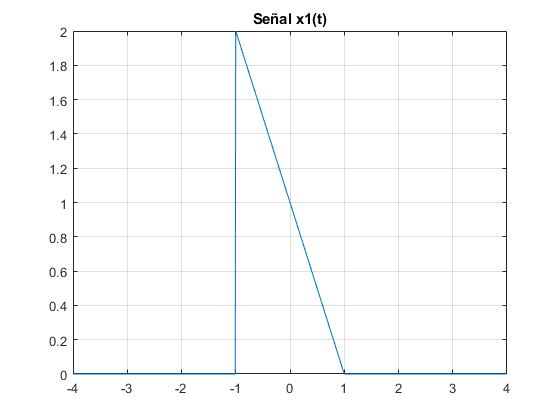
\includegraphics[width=\linewidth]{./Imágenes/aau.png}
\end{subfigure}
\end{figure}

\end{myenumerate}


\setlength{\leftskip}{0pt}
\setlength{\rightskip}{0pt}


\subsubsection{Propiedades de la suma de convolución}
\vspace{\parskip}
\begin{itemize}
\item Propiedad \textbf{conmutativa}. \[x_1[n]*x_2[n]=[x_2[n]*x_1[n] \]
\item Propiedad \textbf{asociativa} (interconexión en cascada).
\item Propiedad \textbf{distributiva} (interconexión en paralelo).
\end{itemize}

\section{Sistemas discretos lineales e invariantes}


\section{Sistemas continuos lineales e invariantes}


\section{Propiedades de los sistemas lineales e invariantes}





\chapter{Análisis de Fourier para señales y sistemas de tiempo continuo}

\section{Introdución al análisis de Fourier}
\subsection{Ecuación en diferencias}

Como vamos a tratar con sistemas LTI, podemos aplicar la propiedad de linealidad para intentar expresar las diferentes señales como una combinación lineal de señales básicas.

En el caso de señales discretas, podemos representar estas señales básicas como:
\begin{align*}
\phi_k[n]  & = \delta [n-k] \\
\psi _k[n] & = h[n-k]
\end{align*}

En el laboratorio, seguramente tengas que trabajar con estas señales en el entorno de MATLAB. Esta es la expresión general de una ecuación en diferencias:

\[\sum^{N}_{k=0}{a_k\cdot y[n-k]} = \sum^{M}_{k=0}{b_k\cdot x[n-k]}\]

\subsection{Uso de la exponencial compleja}

Sin embargo, para tener una señal básica que nos sirva en un caso general, vamos a tomar la \textbf{exponencial compleja}, ya que sus propiedades nos van a ser muy útiles a la hora de operar.
\begin{align*}
&  &  &  &  &  &  &  & \phi_k(t)  & = e^{s_kt} & s_k \equiv \text{nº complejo} &  &  &  &  &  &  &  & \\
&  &  &  &  &  &  &  & \psi _k[n] & = z_k^n    & z_k \equiv \text{nº complejo} &  &  &  &  &  &  &  &
\end{align*}

Veremos que al realizar un análisis de Fourier de estas señales, lo que en realidad estaremos haciendo es analizar las señales \textbf{en términos de exponenciales complejas}:
\begin{align*}
&  &  &  &  &  &  &  & s_k       & = j\omega_k & \longrightarrow  \phi_k(t) & = e^{j\omega_kt} &  &  &  &  &  &  &  & \\
&  &  &  &  &  &  &  & \abs{z_k} & = 1         & \longrightarrow  \phi_k[n] & = e^{j\Omega_kn} &  &  &  &  &  &  &  &
\end{align*}

\section{Señales exponenciales complejas}
Las señales exponenciales complejas son \textbf{autofunciones}. Esto quiere decir que, si la entrada de un sistema es una exponencial compleja de la forma $x(t) = e^{j\omega_ot}$, la salida será: \[y(t) = e^{j \omega _0 t} \H (j\omega _0)\]

Vemos que la salida es exactamente igual que la entrada, pero multiplicada por un factor $\H (j\omega _0)$, denominado \textbf{autovalor}, el cual depende de la frecuencia de la señal de entrada. Esto quiere decir que la salida tendrá la misma forma que la entrada, pero con diferente amplitud.

Por otro lado, podemos ver que si la entrada es una combinación lineal de señales exponenciales... \[x(t) = \sum^{N}_{k=1}{a_ke^{j\omega _kt}}\]

Entonces la salida que obtendremos es también una combinación lineal de exponenciales: \[y(t) = \sum^{N}_{k=1}{b_ke^{j\omega _kt}} \qquad \qquad \left( b_k = a_k \H{\left( j\omega _k \right)} \right)\]

Una vez tengamos las señales en términos de exponenciales complejas, podremos realizar una aproximación diferente según el tipo de señal:
\begin{itemize}
\item Para \textbf{señales periódicas}, estudiaremos las \hyperref[sec:Series_de_Fourier]{series de Fourier}.
\item Para \textbf{señales no periódicas}, estudiaremos la \hyperref[sec:Transformada_de_Fourier]{transformada de Fourier}.
\end{itemize}


\section{Series de Fourier} \label{sec:Series_de_Fourier}

Como trataremos señales periódicas, teniendo una señal $x(t) = e^{j\omega_ot}$, sabemos que:
\begin{align*}
x(t) & = x\left( t-T_o \right) \\
T_o  & = \frac{2\pi}{\omega_o}
\end{align*}

Lo que Fourier descubrió fue que es posible representar cualquier señal periódica como una combinación lineal de señales armónicamente relacionadas.

Si la señal es en realidad $x(t) = e^{jk\omega_ot}$, siendo $k$ un número entero, podemos obtener las señales \textbf{armónicamente relacionadas} dándole a $k$ diferentes valores.
\[\frac{T_o}{k} = \frac{2\pi}{k\omega_o}\]

De esta forma, podemos obtener la forma exponencial compleja de las \textbf{series de Fourier}:
\[\boxed{x(t) = \sum^{+\infty}_{k=-\infty}{a_ke^{jk\omega_ot}}}\]

Nótese que en esta definición existen valores negativos de frecuencia. Esto no resulta una contradicción si interpretamos las frecuencias negativas como un recorrido horario del círculo complejo que representan las exponenciales complejas.

\subsection{Fenómeno de Gibbs}

\section{Transformada de Fourier} \label{sec:Transformada_de_Fourier}
La transformada de Fourier es una particularización de la \textbf{transformada de Laplace} de modo que $s=j\omega$.
\subsection{Definición}
Dada una señal $x(t)$, se define su \textbf{transformada de Fourier} como: \[\boxed{X(\omega ) = \int_{-\infty}^{\infty}{x(t) e^{-j\omega t}dt}}\]

\subsection{Cálculo de los coeficientes}

\section{Transformada de Fourier para señales periódicas}

\section{Respuesta en frecuencia de sistemas continuos. Representación gráfica}

\section{Muestreo ideal}

\section{Aplicación de la Transformada de Laplace al análisis de sistemas LTI}

\section{La función del sistema de sistemas continuos}

\section{Sistemas descritos por ecuaciones diferenciales lineales de coeficientes constantes}

\section{Introducción al filtrado}


\chapter{Análisis de Fourier para señales y sistemas de tiempo discreto}

\section{Respuesta de sistemas discretos LTI a señales exponenciales complejas}

\section{Representación de señales periódicas: la Serie Discreta de Fourier}

\section{Transformada de Fourier para señales no periódicas}

\section{Transformada de Fourier para señales periódicas}

\section{Respuesta en frecuencia de sistemas discretos}

\section{Estudio de señales y sistemas discretos en el dominio transformado Z}

\section{Aplicación de la Transformada Z al análisis de sistemas LTI}

\section{La función de sistema de sistemas discretos}

\section{Sistemas de tiempo discreto descritos por ecuaciones en diferencias lineales de coeficientes constantes}

\section{Introducción al filtrado}


\chapter{Prácticas}

\section{Introducción a Matlab. Representación de Señales}

\section{Convolución}

\section{Análisis de sistemas de tiempo discreto}
La \textbf{función de transferencia} $H(z)$ de uns sistema LTI puede obtenerse de varias formas:
\begin{enumerate}
\item A partir de la transforma Z de su respuesta al impulso.
\[H(z) = \text{TZ}\{ h[n]\} = \sum_{n=-\infty}^{\infty}h[n]z^{-n}\]
\item A partir de las transformadas Z de las señales de entrada y de salida.

\begin{figure}[!ht]
\centering
\begin{tikzpicture}[auto,>=latex']
\node [input, name=input] (input) {$X(z)$};
\node [block, right of=input, node distance=2cm] (controller) {$\quad \begin{matrix} H(z) \\[5pt]\text{LTI} \end{matrix}\quad $};
\node [output, right of=controller, node distance=4cm] (output) {};

\draw [->] (input) -- node{$X(z)$} (controller);
\draw [->] (controller) -- node{$Y(z) = X(z)\cdot  H(z)$} (output);
\end{tikzpicture}
\caption{}
\end{figure}
\end{enumerate}

En la mayor parte de los casos, nos interesará conocer $H(z)$ como el cociente de dos polinomios.
\[H(z) = \frac{b_0 +b_1z^{-1}+b_2z^{-2}+\dots}{a_0 +a_1z^{-1}+a_2z^{-2}+\dots}\]
Las raíces del denominador serán los polos del sistema y las raíces del numerados serán los ceros del sistema.


\appendix
\chapter{Ejercicios del Tema 1}
\begin{ejercicio} \label{ej001}
Se tiene una señal $x(t)$ (véase la figura ...) y se quiere construir una señal $y(t) =x(2t+2)$.
\end{ejercicio}
\textbf{Solución:} En este tipo de ejercicios, la primera operación que tenemos que aplicar es el desplazamiento. Luego aplicaremos el resto.

\chapter{Ejercicios del Tema 2}
\chapter{Ejercicios del Tema 3}
\chapter{Ejercicios del Tema 4}


%%% FIN DE LOS APUNTES %%%

%%% BIBLIOGRAFÍA %%%
% Por defecto, se encuentra desactivada. Esto disminuye el tiempo de procesado. Se puede activar cuando se vaya a exportar el PDF definitivo

% \newpage
% \phantomsection
% \label{sec:bibliografia_final}
% \renewcommand{\refname}{Bibliografía} % Para cambiar el título al incluir una librería de BibTeX
% \addcontentsline{toc}{section}{Bibliografía}
% \bibliographystyle{ieeetr}
% \bibliography{biblio_tex.bib}

\end{document}
